% !TEX root = ../my-thesis.tex
%
\chapter{Data Analysis}
\label{sec:analysis}
In this chapter the models calculated for each country are reviewed. First, a look at the standardised incidence rate for each country is taken, before spatial models, spatio-temporal models and finally predictive models are discussed.
\section{Standardised Incidence Ratio}
This section takes a brief look at the standardised incidence ratio for the countries of interest.
\subsection{Standardised Incidence Ratio for Germany}
When looking at the standardised incidence ratio for Germany, it is noticeable that the actual number of infections in the eastern parts of Germany, especially in Saxony, is considerably higher than the expected number of infections. Furthermore, parts of Bavaria have an increased standardised incidence ratio compared to the rest of Germany, excluding Saxony. This could be due to the fact that the regions share a border with the Czech Republic, a country that is substantially more affected by Covid-19 than Germany. The northern parts of Germany show the lowest SIR which is possibly due to the fact that this region is sparsely populated. For more information, see Figure~\ref{sirgermany}.
% \begin{figure}[H]
%   \centering
%   \includesvg[width = 1.2\textwidth]{sir_germany.svg}
%   \caption{The standardised incidence ratio for Germany based on the data of the 18th of March 2021}
%   \label{sirgermany}
% \end{figure}
\begin{figure}[H]
  \centering
  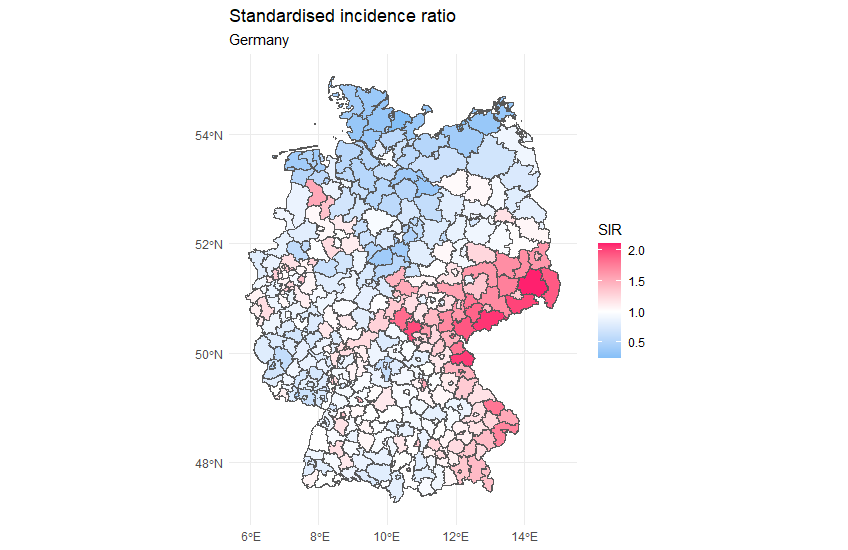
\includegraphics[width = 1.2\textwidth]{sir_germany.png}
  \caption{The standardised incidence ratio for Germany based on the data of the 18th of March 2021}
  \label{sirgermany}
\end{figure}
\subsection{Standardised Incidence Ratio for Norway}
Looking at the standardised incidence rate for Norway, a standardised incidence rate of less than 1 can be seen for most municipalities north of Trondheim. In the southern parts of Norway there are several municipalities with a rate above 1, for example the standardised incidence rate around the capital Oslo is around 2. However, the two small municipalities, Hyllestad and Ulvik, have the highest standardised incidence rate in Norway. In Hyllestad, 95 of 1328 people have been infected with Covid-19 so far, while in Ulvik, 134 of 1080 people have been infected so far. \\
The SIR in Hyllestad is around 4.5, following an outbreak in a shipyard in autumn 2020 \cite{newspaper1}, while Ulvik has a ratio of around 8, following an outbreak of the UK variant of Covid-19. According to the head of the municipality, Hans Petter Thorbjørnsen, the infections are thought to have spread through children \cite{newspaper2}. See Figure~\ref{sirnorway} for more information.
% \begin{figure}[H]
%   \centering
%   \includesvg[width = 1.2\textwidth]{sir_norway.svg}
%   \caption{The standardised incidence ratio for Norway based on the data of the 20th of March 2021}
%   \label{sirnorway}
% \end{figure}
\begin{figure}[H]
  \centering
  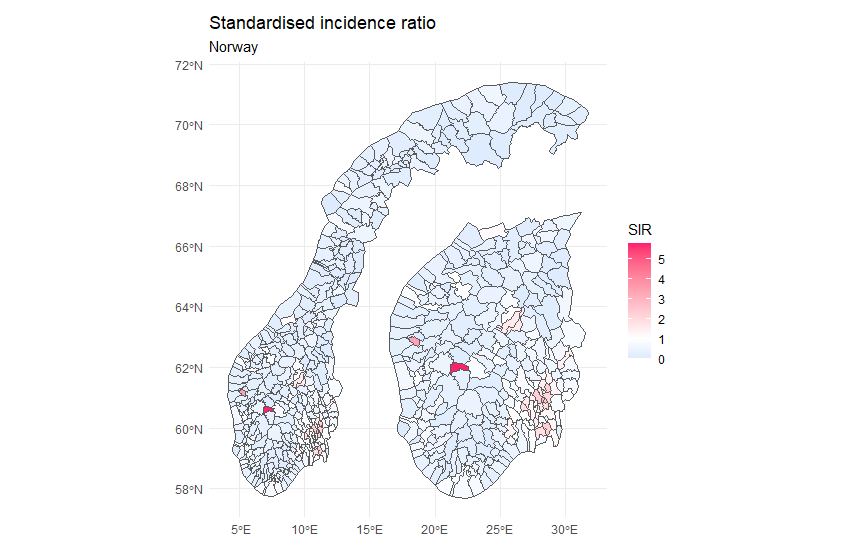
\includegraphics[width = 1.2\textwidth]{sir_norway.png}
  \caption{The standardised incidence ratio for Norway based on the data of the 20th of March 2021}
  \label{sirnorway}
\end{figure}
Because the high numbers from two small municipalities complicate the interpretation of Figure~\ref{sirnorway}, Figure~\ref{sirnorwaylog} shows the SIR on a log10 scale. It is now clearer that the standardized incidence ratio is below 1 in most parts of Norway, but that there is a higher risk in the region around Oslo.
% \begin{figure}[H]
%   \centering
%   \includesvg[width = 1.2\textwidth]{sir_norway_log.svg}
%   \caption{The log10 standardised incidence ratio for Norway based on the data of the 20th of March 2021}
%   \label{sirnorway}
% \end{figure}
\begin{figure}[H]
  \centering
  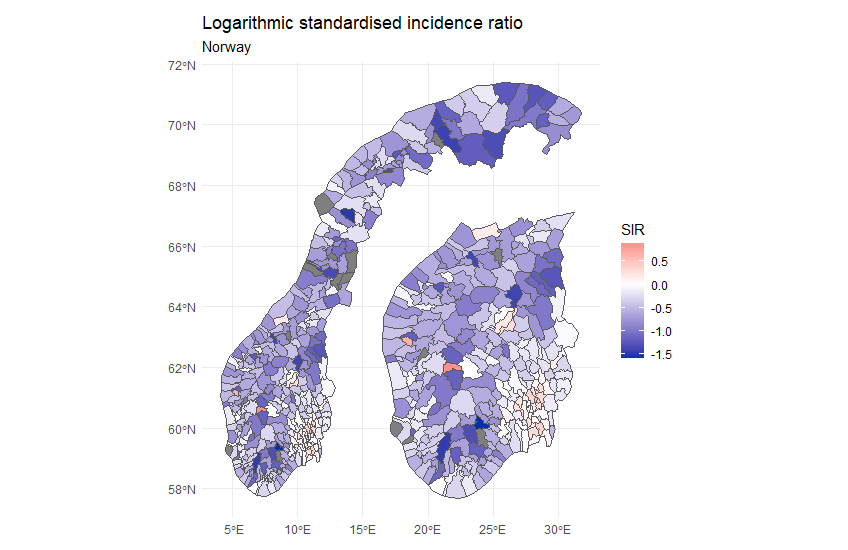
\includegraphics[width = 1.2\textwidth]{sir_norway_log.png}
  \caption{The log10 standardised incidence ratio for Norway based on the data of the 20th of March 2021}
  \label{sirnorwaylog}
\end{figure}
\clearpage
\section{Spatial Models}
After looking at the standardised incidence rates for the countries of interest, the next step is to take a closer look at the current figures for the respective countries. Spatial models are used to try to extract the factors that cause some populations to be at higher risk than other populations. Three different types of models are used for each country:
\begin{itemize}
    \item[1.] The Besarg-Yollie-Mollie Model
    \item[2.] Besags Proper Spatial Model
    \item[3.] The Leroux-Model
\end{itemize}
All of these models were computed using the INLA \cite{rinla} R package. \\
To specify each type of model, the code shown in Listing~\ref{codeModels} can be used. \\
Three measures are used to compare the models, the DIC, the WAIC and the CPO. \\
For all countries, the models were computed with
\begin{itemize}
    \item[1.] only the demographic variables as covariates
    \item[2.] only the infrastructural variables as covariates
    \item[3.] both, demographic and infrastructural variables, as covariates
    \begin{itemize}
        \item[3.1] Without variable selection
        \item[3.2] With variable selection
    \end{itemize}
\end{itemize}
For each model type, different values for the penalised prior were tried. As this resulted in a large number of models, only the model with the best performance for each model class is examined in more detail. \\
The models were compared using the mean absolute error. For this, 20\% of the observations were removed from the training and used for testing instead. The predicted number of infections for these municipalities was then compared to the actual numbers.
\\
Finally, due to the amount of covariates, forwards and backwards stepwise variable selection was performed with the intention of obtaining a model that fits the data well and at the same time is relatively easy to interpret. This can be done with the R package \texttt{INLAutils} \cite{inlautils}, as shown in Listing~\ref{codeSelection}. Backwards as well forwards variable selection was performed.\\
A list of all calculated models along with their performance measures is provided in the appendix.
\subsection{Model Selection}
Before the models are computed, however, the distribution that fits the number of cases must first be found. For this, the function \texttt{descdist()} from the \texttt{fitdistrplus} R package is used. The Cullen and Frey graph can be used to give an initial idea of which distributions fit the data, in this case the number of infections, reasonably well depending on the kurtosis and the square of the skewness. \\
The plots for Germany and Norway can be seen in Figure~\ref{cf_germany} and Figure~\ref{cf_norge}.
% \begin{figure}[H]
%     \centering
%     \includesvg[width = 0.8\textwidth]{cf_germany.svg}
%     \caption{The Cullen and Frey graph for Germany}
%     \label{cf_germany}
% \end{figure}
\begin{figure}[H]
    \centering
    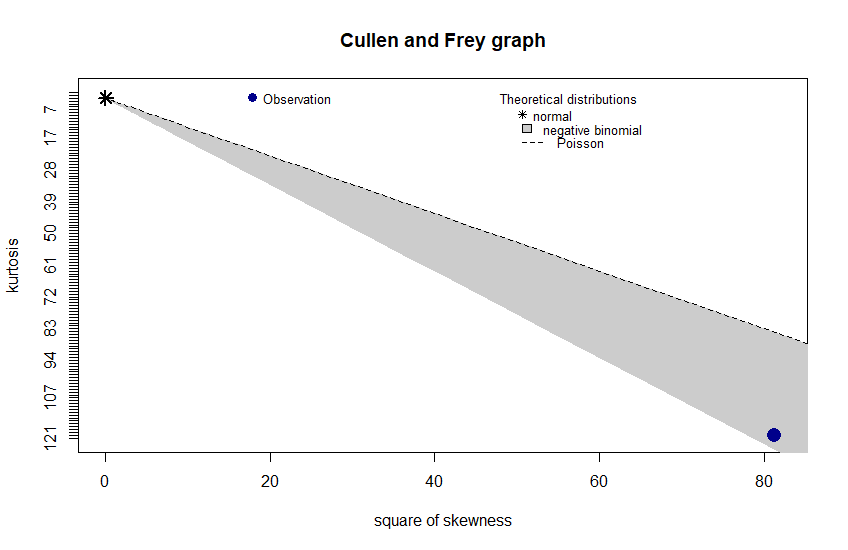
\includegraphics[width = 0.8\textwidth]{cf_germany.png}
    \caption{The Cullen and Frey graph for Germany}
    \label{cf_germany}
\end{figure}
% \begin{figure}[H]
%     \centering
%     \includesvg[width = 0.8\textwidth]{cf_norge.svg}
%     \caption{The Cullen and Frey graph for Norway}
%     \label{cf_norge}
% \end{figure}
\begin{figure}[H]
    \centering
    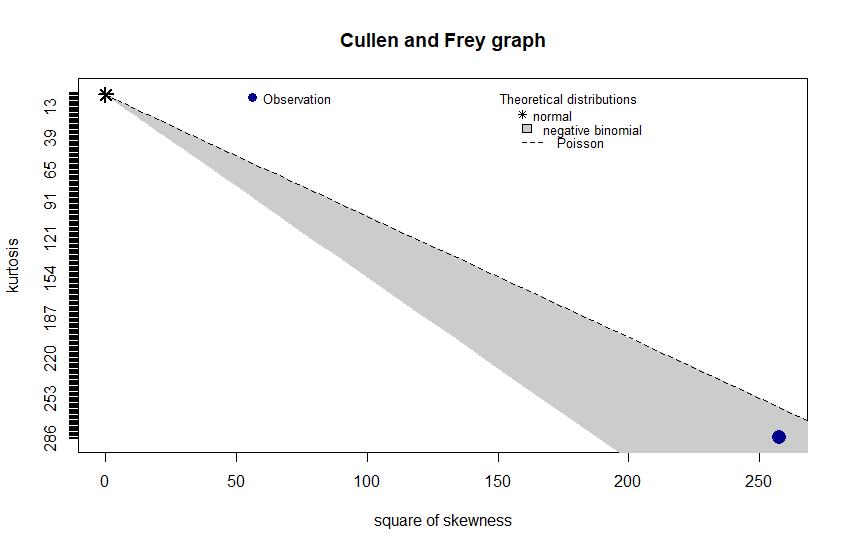
\includegraphics[width = 0.8\textwidth]{cf_norge.png}
    \caption{The Cullen and Frey graph for Norway}
    \label{cf_norge}
\end{figure}
Next, a negative binomial distribution, a normal distribution, and a Poisson distribution are fitted to the data using the maximum likelihood method. The negative binomial fits for both countries can be seen in Figure~\ref{fitNegbinomGermany} and Figure~\ref{fitNegbinomNorway}. The fits for the normal and Poisson distribution for both countries, are shown in the Appendix in Figure~\ref{fitNormalGermany}, Figure~\ref{fitPoissonGermany}, Figure~\ref{fitNormalNorway} and Figure~\ref{fitPoissonNorway}.
% \begin{figure}[H]
%     \centering
%     \includesvg[width = 0.8\textwidth]{fit_nbinom_germany.svg}
%     \caption{A negative binomial fit to the number of cases in German municipalities}
%     \label{fitNegbinomGermany}
% \end{figure}
\begin{figure}[H]
    \centering
    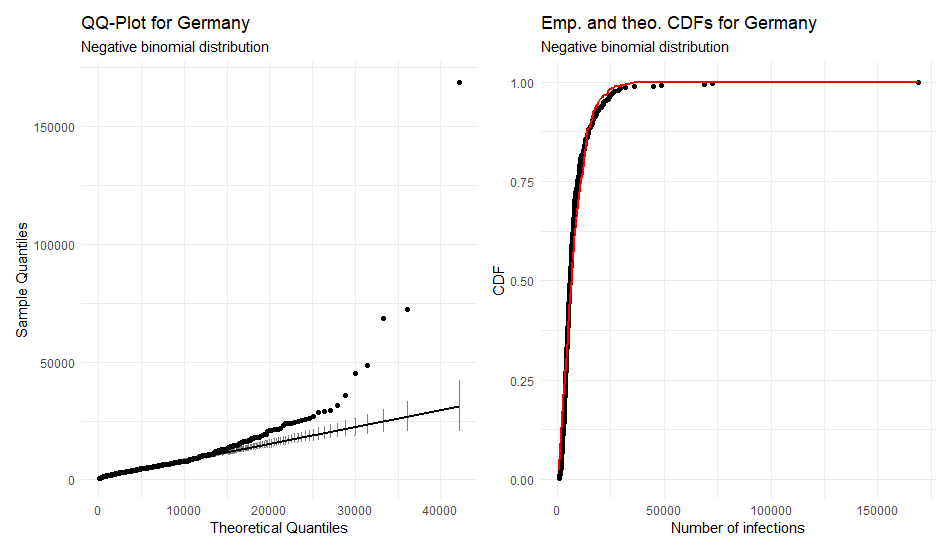
\includegraphics[width = 0.8\textwidth]{fit_nbinom_germany.png}
    \caption{A negative binomial fit to the number of cases in German municipalities}
    \label{fitNegbinomGermany}
\end{figure}
% \begin{figure}[H]
%     \centering
%     \includesvg[width = 0.8\textwidth]{fit_nbinom_norway.svg}
%     \caption{A negative binomial fit to the number of cases in Norwegian municipalities}
%     \label{fitNegbinomNorway}
% \end{figure}
\begin{figure}[H]
    \centering
    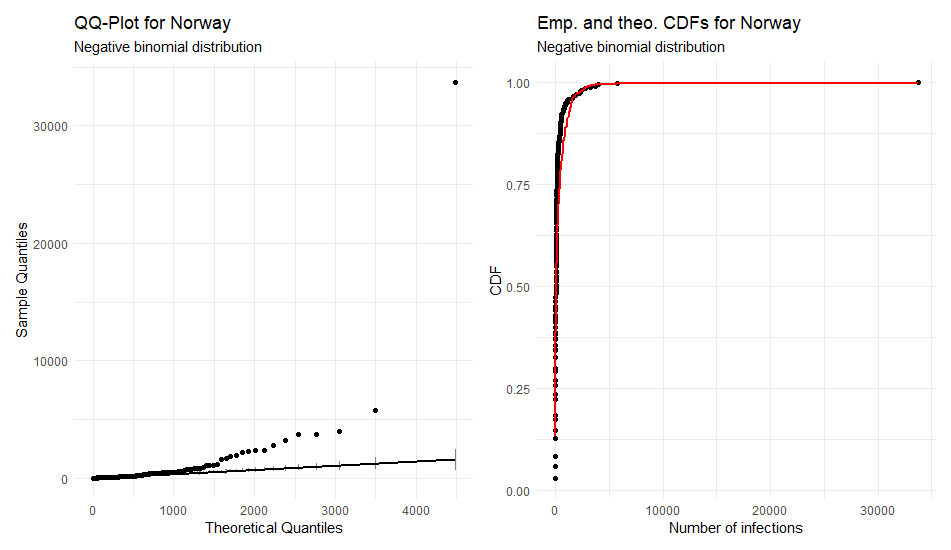
\includegraphics[width = 0.8\textwidth]{fit_nbinom_norway.png}
    \caption{A negative binomial fit to the number of cases in Norwegian municipalities}
    \label{fitNegbinomNorway}
\end{figure}
Lastly, the AIC was calculated for fitting a normal distribution to the data, a Poisson distribution to the data and a negative binomial distribution to the data. The values can be seen in Table~\ref{aic}. Afterwards, the negative binomial distribution was chosen as the distribution of the target variable in both cases. \\
\begin{table}[H] 
\caption{The AIC for different distributions for Germany and Norway \label{aic}}
\begin{tabular}{l l r}
\toprule
\textbf{Country}	& \textbf{Distribution}	& \textbf{AIC} \\
\midrule
Germany & Normal & 8360 \\
Germany & Poisson & 2148100 \\
Germany & Negative Binomial & 7731 \\
Norway & Normal & 6166 \\
Norway & Poisson & 366181 \\
Norway & Negative Binomial & 4086 \\
\bottomrule
\end{tabular}
\end{table} 
The poor fit for the Poisson distribution can be explained by looking at the range of the number of confirmed cases in a given municipality. For Germany, this number ranges from 508 to 137634 (as of March 18, 2021), while for Norway, the number ranges from 0 to 24905 (as of March 20, 2021). This results in a mean and standard deviation for Germany of 6617 and 9014, respectively. For Norway, the values for these metrics are 236 and 1389.
\subsection{Spatial Models for Germany}
First, a look is taken at the spatial models calculated for Germany. These models are based on data from 18 March 2021, when 2.669.233 people in Germany were confirmed infected with Covid-19. The five municipalities with the most infections are shown in Table~\ref{top5germany}.
\begin{table}[H] 
\caption{The municipalities with the most infections as of March 18th 2021. \label{top5germany}}
\begin{tabular}{l r r}
\toprule
\textbf{Municipality}	& \textbf{Population}	& \textbf{Number of infections} \\
\midrule
SK Berlin & 3644826 & 137634 \\     
SK Hamburg & 1841179 & 56656 \\
SK Munich & 1471508 & 56559 \\
SK Cologne & 1085664 & 36455 \\
Region Hannover & 1157624 & 35097 \\
\bottomrule
\end{tabular}
\end{table}
\subsubsection{Demographic Models}\label{sssec:demoGermany}
The model with the best performance based on the demographic variables was a Leroux model calculated formula in Listing~\ref{codeDemoGermany}. The variables used for this model were the percentages of the vote for the six biggest German political parties. \\
The performance measures of this model and the best-performing BYM2 and Besag proper models are shown in Table~\ref{demoGermany}. 
\begin{table}[H] 
\caption{The performance measures for the best performing demographic model of each type. \label{demoGermany}}
\begin{tabular}{l r r r r}
\toprule
\textbf{Model}	& \textbf{DIC}	& \textbf{WAIC} & \textbf{CPO} & \textbf{MAE}\\
\midrule
Besag  & 4598 & 4598 & -2715 & 219618 \\
BYM2 & 4535 & 4502 & -2704 & 219109\\
Leroux & 4685  & 4716 & -2976 & 216908\\
\bottomrule
\end{tabular}
\end{table}
The summary of the fixed effects is shown in Table~\ref{fixedDemoGermany}. To compute the posterior mean of the coefficients, the code shown in Listing~\ref{codePosteriorMean} can be used. \\
To obtain a credibility interval of the fixed effects on the transformed scale, the code in Listing~\ref{codeCredibility} can be used. \\
\begin{table}[H] 
\caption{The fixed effects for the Leroux model. Values are rounded. \label{fixedDemoGermany}}
\begin{tabular}{l r r r r}
\toprule
\textbf{Variable}	& \textbf{Mean}	& \textbf{exp(mean$_{\hbox{p}}$)} & \textbf{exp(q0025$_{\hbox{p}}$)} & \textbf{exp(q0975$_{\hbox{p}}$)} \\
\midrule
(Intercept) & -0.07733 & 0.9257 & 0.8953 & 0.9568 \\
Union & -0.1307 & 0.8804 & 0.7485 & 1.029 \\
SPD & -0.1597 & 0.8531 & 0.7842 & 0.9264 \\
Gruene & -0.1055 & 0.9022 & 0.7812 & 1.036 \\
FDP & 0.001426 & 1.002 & 0.9630 & 1.041 \\
die\_linke & -0.1930 & 0.8254 & 0.7505 & 0.9057 \\
afd & 0.1377 & 1.150 & 1.005 & 1.311 \\
\bottomrule
\end{tabular}
\end{table}
The posterior mean of the exponentiated intercept implies a -7.43\% risk rate across Germany with a credibility interval ranging from -10.47\% to 4.32\%.  \\
This summary shows that especially people who come from regions where the AfD gets a higher share of the vote have a higher risk of contracting Covid-19. In Figure~\ref{sirgermany}, regions in eastern Germany often had a higher SIR. These are also the regions where the AfD tends to perform better in elections. The connection between the two can be attributed to the fact that the AfD is a right-wing party that openly criticises the measures taken to prevent the spread of the coronavirus. As a result, a large proportion of people who vote for the AfD do not take the measures seriously either and refuse to keep a safe distance or wear a mask in public spaces. \\
A one standard deviation increase for the AfD leads to a risk increase of about 15\%. The only other party with a posterior mean greater than 1 is the liberal FDP, which is known for its capitalist views. An increase of one standard deviation increases the risk by 0.16\%. \\
As for the rest of the parties, they are either the leading party in Germany (Union) or left-wing oriented (SPD, the Greens and the Left). People who vote for left-wing parties may respect the Corona rules more and show more consideration for other people.
As this was the overall best-performing spatial model for Germany, a look is taken at the posterior means $\pmb{\zeta} = \exp{\left(\xi\right)}$ of the area-specific risks. Since the uncertainty associated with them can also be mapped, the posterior probability $\mathbb{P}\left(\zeta_i > 1|y\right)$ is visualised as well. In Figure~\ref{posteriorGermany} it can be seen that the relative risk is higher in the south-eastern parts of Bavaria as well as in parts of Saxony, North Rhine-Westphalia and Brandenburg. The posterior probability for these regions is mostly between 0.75 and 1. Both Saxony and Brandenburg are political strongholds for the AfD, while North Rhine-Westphalia is home to the Ruhr region, Germany's most populous metropolitan area. The higher numbers in Bavaria can be explained by the large common borders with Austria and the Czech Republic, two countries that were more affected by the pandemic. Many people cross these borders because of tourism and many guest workers come from the Czech Republic to work on agricultural land in Bavaria, which resulted in several Covid-19 outbreak events.
\begin{figure}[H]
    \centering
    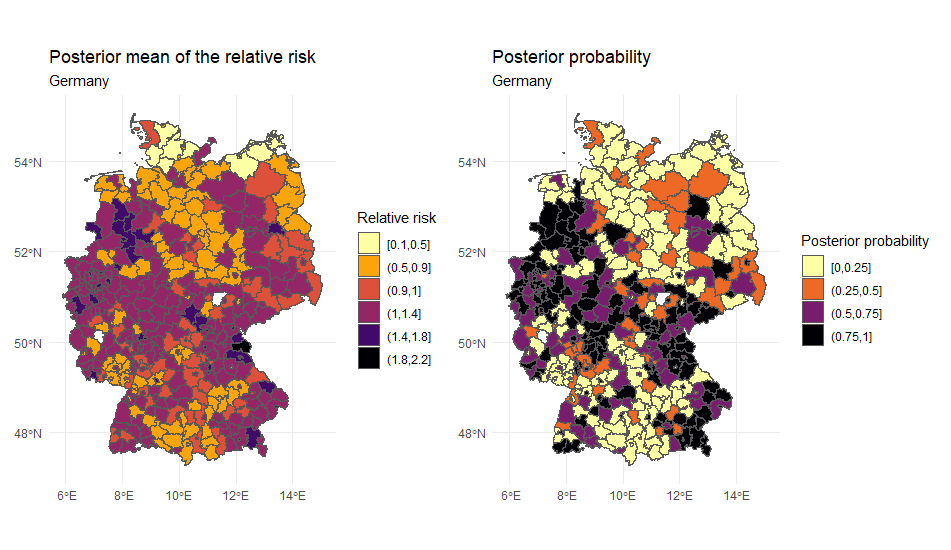
\includegraphics[width = \textwidth]{posterior_germany.png}
    \caption{Posterior mean of the area-specific risk and the posterior probability.}
    \label{posteriorGermany}
\end{figure}
% \begin{figure}[H]
%     \centering
%     \includesvg[width = textwidth]{posterior_germany.svg}
%     \caption{A negative binomial fit to the number of cases in Norwegian municipalities}
%     \label{nb_norge}
% \end{figure}
\subsubsection{Infrastructure Models}
When it comes to the models based on the infrastructural variables, a BYM2 model performed the best. It was computed using formula in Listing~\ref{codeInfraGermany}. \\
The performance measures of this model and the best-performing Besag proper and Leroux model are shown in Table~\ref{infraGermany}
\begin{table}[H] 
\caption{The performance measures for the best performing demographic model of each type. \label{infraGermany}}
\begin{tabular}{l r r r r}
\toprule
\textbf{Model}	& \textbf{DIC}	& \textbf{WAIC} & \textbf{CPO} & \textbf{MAE}\\
\midrule
Besag & 4604 & 4598 & -2742 & 232444\\
BYM2 & 4561 & 4539 & -2714 & 230728\\
Leroux & 4727 & 4754 & -3318 & 238526\\
\bottomrule
\end{tabular}
\end{table}
The values of the covariates are shown in Table~\ref{fixedInfraGermany}.
\begin{table}[H] 
\caption{The fixed effects for the BYM2 model. Values are rounded. \label{fixedInfraGermany}}
\begin{tabular}{l r r r r}
\toprule
\textbf{Variable}	& \textbf{Mean}	& \textbf{exp(mean$_{\hbox{p}}$)} & \textbf{exp(q0025$_{\hbox{p}}$)} & \textbf{exp(q0975$_{\hbox{p}}$)} \\
\midrule
(Intercept) & -0.07275 & 0.9299 & 0.9168 & 0.9430 \\
shops & 0.1590 & 1.179 & 0.9487 & 1.448 \\
hairdresser & 0.1554 & 1.172 & 1.003 & 1.360 \\
marketplace & 0.03241 & 1.034 & 0.9663 & 1.104 \\
schools & 0.03174 & 1.034 & 0.9325 & 1.143 \\
nursing\_home & 0.006124 & 1.006 & 0.9775 & 1.036 \\
bakeries & 0.005910 & 1.009 & 0.8563 & 1.181 \\
place\_of\_worship & 0.001925 & 1.002 & 0.9591 & 1.047 \\
entertainment & -0.01105 & 0.9907 & 0.8812 & 1.110 \\
retail & -0.01147 & 0.9892 & 0.9235 & 1.058 \\
aerodrome & -0.01204 & 0.9884 & 0.9368 & 1.042 \\
sport & -0.01208 & 0.9888 & 0.9151 & 1.067 \\
higher\_education & -0.02014 & 0.9803 & 0.9420 & 1.020 \\
office & -0.03995 & 0.9615 & 0.8942 & 1.032 \\
platform & -0.04970 & 0.9519 & 0.8971 & 1.009 \\
clinic & -0.05596 & 0.9460 & 0.8929 & 1.001 \\
kindergarten & -0.09283 & 0.9143 & 0.7797 & 1.065 \\
restaurant & -0.1094 & 0.8984 & 0.7877 & 1.020 \\
\bottomrule
\end{tabular}
\end{table}
Some findings from these results are that shops, defined as supermarkets, convenience stores and drugstores, hairdressers, marketplaces, schools, nursing homes, bakeries and places of worship all increase the risk of infection. The two highest are shops and hairdressers, where a 1 standard deviation increase leads to a 17.9\% increase in risk in the case of shops and a 17.2\% increase in risk for hairdressers. It should not be surprising that shops in particular increase the risk of infection, as people tend to congregate there and people living in areas where a supermarket is nearby may prefer to go shopping more often to buy fresh produce rather than just once a week when a supermarket is further away. \\
In Germany, there was a big discussion about whether hairdressers should be allowed to stay open during lockdowns, as they were forced to close and could only work when there was no lockdown. Seeing how much hairdressers increase the risk of infection, it might have been a wise decision not to allow them to continue working during a closure. \\
Finally, the number of schools in a given community also increases the risk of infection. An increase of 1 standard deviation increases the risk by about 3.4\%.
\\
There are also effects that have a posterior mean of less than 1, suggesting that they reduce the risk of infection. However, this is not necessarily the case, as it is probably safer for a person to stay at home than to go to a restaurant, for example. It is interesting to note, however, that the lowest posterior mean was observed for restaurants. This could be due to the fact that during most of the time restaurants were either only allowed to serve take-away food or had very strict hygiene policies. The low value could indicate that these measures worked as intended.
\subsubsection{Combined Models}
Finally, models are considered that include both the infrastructural and demographic covariates. Due to the amount of variables, all models run are based on variable selection. \\
The best performing model was again a BYM2 model, run with the formula shown in Listing~\ref{codeBothGermany}. \\
The performance measures of the computed models are shown in Table~\ref{allGermany}.
\begin{table}[H] 
\caption{The performance measures for the best performing demographic model of each type. \label{allGermany}}
\begin{tabular}{l r r r r}
\toprule
\textbf{Model}	& \textbf{DIC}	& \textbf{WAIC} & \textbf{CPO} & \textbf{MAE}\\
\midrule
Besag&  4628 & 4605 & -2673 & 249901\\
BYM2 & 4580 & 4571 & -2683 & 247323\\
Leroux & 4764 & 4791 & -2833 & 248031 \\
\bottomrule
\end{tabular}
\end{table}
The fixed effects are shown in Table~\ref{fixedAllGermany}.

\begin{table}[H] 
\caption{The fixed effects for the BYM2 model. Values are rounded. \label{fixedAllGermany}}
\begin{tabular}{l r r r r}
\toprule
\textbf{Variable}	& \textbf{Mean}	& \textbf{exp(mean$_{\hbox{p}}$)} & \textbf{exp(q0025$_{\hbox{p}}$)} & \textbf{exp(q0975$_{\hbox{p}}$)} \\
\midrule
(Intercept) & -0.07327 & 0.9294 & 0.9149 & 0.9438 \\
afd & 0.2488 & 1.283 & 1.213 & 1.356 \\
pop\_dens & 0.1196 & 1.127 & 1.078 & 1.178 \\
schools & 0.04867 & 1.051 & 0.9586 & 1.150 \\
welfare\_recipients & 0.04565 & 1.048 & 0.9579 & 1.143 \\
sport & 0.02466 & 1.026 & 0.9586 & 1.096 \\
place\_of\_worship & -0.0002002 & 1.000 & 0.9633 & 1.038 \\
nursing\_home & -0.0006482 & 0.9994 & 0.9752 & 1.024 \\
kindergarten & -0.002457 &  0.9993 & 0.8898 & 1.119 \\
log(trade\_tax) & -0.006766 & 0.9933 & 0.9705 & 1.016 \\
FDP & -0.01635 & 0.9840 & 0.9453 & 1.024 \\
office & -0.01770 & 0.9830 & 0.9178 & 1.051 \\
bakeries & -0.02426 & 0.9780 & 0.8627 & 1.1104 \\
platform & -0.03003 & 0.9708 & 0.9186 & 1.025 \\
entertainment & -0.04251 & 0.9594 & 0.8763 & 1.048 \\
SPD & -0.05188 & 0.9497 & 0.9088 & 0.9919 \\
die\_linke & -0.1284 &  0.8799 & 0.8288 & 0.9333\\
\bottomrule
\end{tabular}
\end{table}
According to this model, the three biggest driving factors are the percentage of votes the AfD receives, the population density and the number of schools in a municipality. The influence of the AfD and the number of schools has already been discussed in section~\ref{sssec:demoGermany}. Regarding population density, it can be said that if it increases by 1 standard deviation, the risk of infection increases by 12.7\%. The more people are concentrated per square kilometre, the easier it is for a virus to spread because the distances between people become smaller. Other factors that positively influence the risk of infection are the number of social welfare recipients, the number of sports facilities and the number of places of worship, although the risk increase for the latter is only just above 0. Sports facilities are again a place where many people come together, and here, depending on the type of sport, there can also be more contact, which in turn favours the spread of a virus. The last effect worth mentioning is the logarithmic business tax. If a region receives more revenue through business tax, the risk of infection in that region decreases. Therefore, people in communities where there is less money are at higher risk. 
\subsection{Spatial Models for Norway}
Next, the same types of models are evaluated for Norway. These models are based on data from 12 March 2021, when 76577 people in Norway were confirmed infected with Covid-19. The five municipalities with the most infections are shown in Table~\ref{top5norway}.
\begin{table}[H] 
\caption{The municipalities with the most infections as of March 12th 2021. \label{top5norway}}
\begin{tabular}{l r r}
\toprule
\textbf{Municipality}	& \textbf{Population}	& \textbf{Number of infections} \\
\midrule
Oslo & 693494 & 22248 \\
Bergen & 283929 & 4618 \\
Drammen & 101386 & 2549 \\
Lillestrøm & 85983 & 2390 \\
Fredrikstad & 82385 & 2373 \\
\bottomrule
\end{tabular}
\end{table}
\subsubsection{Demographic Models}
As with Germany, the best demographic model was again a Leroux model. Only this time, the covariates of the model were selected using forwards variable selection. The following formula was used for the model:
\begin{lstlisting}[caption={The formula for the best Leroux model based on the demographic variables}, label={codeDemoNorway}, language = R]
formula_22_leroux <- value ~
  pop_dens + immigrants_pure + median_age +
  sex +
  f(
    idarea_1, model = "generic1",
    Cmatrix = C, hyper = prior_2
  )
\end{lstlisting}
The performance measures for all three types of models are shown in Table~\ref{demoNorway}.
\begin{table}[H] 
\caption{The performance measures for the best performing demographic model of each type. \label{demoNorway}}
\begin{tabular}{l l l l}
\toprule
\textbf{Model}	& \textbf{DIC}	& \textbf{WAIC} & \textbf{CPO} \\
\midrule
Besags Proper  & 2804 (45) & 2820 (45) & -10433 (23) \\
BYM2 & 2716 (3) & 2670 (14) & -9786 (25)\\
Leroux & 2703 (1) & 2648 (1) & -11077 (14) \\
\bottomrule
\end{tabular}
\end{table}
The Leroux model had the best performance in terms of both DIC and WAIC and also performed well in terms of CPO. Just like for Germany, a total of 66 models were calculated. Of the 14 best models in terms of CPO, 13 were Leroux models. \\
The effects of the covariates are shown in Table~\ref{fixedDemoNorway}.
\begin{table}[H] 
\caption{The fixed effects for model 22. Values are rounded. \label{fixedDemoNorway}}
\begin{tabular}{l r r r r}
\toprule
\textbf{Variable}	& \textbf{Mean}	& \textbf{exp(mean$_{\hbox{p}}$)} & \textbf{exp(q0025$_{\hbox{p}}$)} & \textbf{exp(q0975$_{\hbox{p}}$)} \\
\midrule
(Intercept) & 1.087 & 222.4 & -8.203e+09 & -9.140e+04\\
pop\_dens & 0.001775 & 1.002 & 1.001 & 1.003\\
immigrants\_pure & -0.03358 & 0.9671 & 0.9392 & 0.9948\\
median\_age & -0.03628  & 0.9645 & 0.9396 & 0.9897\\
sex & -0.0426 & 2.902e+06 & -6.904e+26 & -1.164e+22 \\
\bottomrule
\end{tabular}
\end{table}
There is little meaningful interpretation for the posterior mean of the intercept in this model due to its high value. Of note is that if the population density increases by 100 persons per square kilometre, the risk of infection increases by about 19.4\%. Furthermore, if the proportion of women in an area increases by 0.05, the risk of infection increases by around 7.7\%. Finally, if the average age in a community increases by 1 year, the risk of infection decreases by roughly 3.5\%. Because younger people tend to be more mobile, they come into contact with more people than older generations, so it makes sense that people living in younger areas have a higher risk of becoming infected with Covid-19.
\subsubsection{Infrastructure Models}
Looking at the 24 models computed for Norway that are based on the infrastructural variables, once again a Leroux model based on forwards variable selection had the best performance. The formula is shown in Listing~\ref{codeInfraNorway}.
\begin{lstlisting}[caption={The formula for the best Leroux model based on the infrastructural variables}, label={codeInfraNorway}, language = R]
formula_30_leroux <- value ~
  pop_dens + shops + retail + place_of_worship +
  schools + nursing_home + kindergarten +
  f(
    idarea_1, model = "generic1",
    Cmatrix = C, hyper = prior_2
  )
\end{lstlisting}
The performance measure for the models are shown in Table~\ref{infraNorway}.
\begin{table}[H] 
\caption{The performance measures for the best performing demographic model of each type. \label{infraNorway}}
\begin{tabular}{l l l l}
\toprule
\textbf{Model}	& \textbf{DIC}	& \textbf{WAIC} & \textbf{CPO} \\
\midrule
Besags Proper  & 2816 (17) & 2813 (17) & -10347 (8) \\
BYM2 & 2728 (2) & 2671 (2) & -9145 (14)\\
Leroux & 2718 (1) & 2665 (1) & -9553 (11) \\
\bottomrule
\end{tabular}
\end{table}
The effect of the covariates are shown in Table~\ref{fixedInfraNorway}.
\begin{table}[H] 
\caption{The fixed effects for model 30. Values are rounded. \label{fixedInfraNorway}}
\begin{tabular}{l r r r r}
\toprule
\textbf{Variable}	& \textbf{Mean}	& \textbf{exp(mean$_{\hbox{p}}$)} & \textbf{exp(q0025$_{\hbox{p}}$)} & \textbf{exp(q0975$_{\hbox{p}}$)} \\
\midrule
(Intercept) & -0.7263 & 0.4858 & 0.4024 & 0.5816 \\
nursing\_home & 0.2017 & 1.270 & 0.7174 & 2.081 \\
retail & 0.1541 & 1.169 & 1.023 & 1.329 \\
kindergarten &  0.07385  &  1.082 & 0.8940 & 1.295 \\
pop\_dens & 0.001853 & 1.002 & 1.001 & 1.003 \\
schools & -0.1022 & 0.9065 & 0.7564 & 1.076 \\
place\_of\_worship & -0.1098 & 0.8987 & 0.7710 & 1.040 \\
shops & -0.1509 & 0.8633 & 0.7228 & 1.022 \\
\bottomrule
\end{tabular}
\end{table}
The posterior mean of the exponential intercept implies a risk rate of -51.42\% across Norway, with a credibility interval ranging from -59.76\% to -41.84\%. However, the risk rate increases if the number of nursing homes per 1000 inhabitants (between 0 and 1.851), retail shops per 1000 inhabitants (between 0 and 10.72), kindergartens per 1000 inhabitants (between 0 and 5.051) or the population density (between 0.1479 and 1437) increases. A 0.1 increase in nursing homes increases the risk by 2.4\%, an increase of 0.1 retail shops per 1000 inhabitants increases the risk by 1.6\% and an increase of 0.1 kindergartens per 1000 inhabitants increases the risk by 0.8\%. Finally, if the population density increases by 50 persons per square kilometre, the risk of infection increases by 20.4\%. Again, there are covariates that negatively affect the risk rate, but as stated earlier, it is probably safer to stay at home than to attend these facilities.
\subsubsection{Combined Models}
Looking at the models with both types of variables for Norway, a BYM2 model that used backwards variable selection performed the best. Its formula can be seen in Listing~\ref{codeAllNorway}
\begin{lstlisting}[caption={The formula for the best BYM2 model based all variables}, label={codeAllNorway}, language = R]
formula_31_bym2 <- value ~
  median_age + unemp_tot + unemp_immg + workers_ft_com + 
  workers_pt_com + mining_ft_com + mining_pt_com +
  construction_pt_com + immigrants_total + immigrants_norge +
  immigrants_pure + marketplace + entertainment + clinic + 
  hairdresser + shops + place_of_worship + retail + 
  nursing_home + aerodrome + platform + kindergarten + 
  schools + bakeries + higher_education + pop_dens + urb_dens +
  f(
    idarea_1, model = "BYM2", graph = g,
    scale.model = TRUE, hyper = prior_1
  )
\end{lstlisting}
In Table~\ref{allNorway}, the performance measure of the respective models can be seen.
\begin{table}[H] 
\caption{The performance measures for the best performing demographic model of each type. \label{allNorway}}
\begin{tabular}{l l l l}
\toprule
\textbf{Model}	& \textbf{DIC}	& \textbf{WAIC} & \textbf{CPO} \\
\midrule
Besags Proper  & 2926 (9) & 2958 (9) & -5811 (9) \\
BYM2 & 2711 (1) & 2673 (2) & -9609 (4)\\
Leroux & 2734 (6) & 2666 (1) & -12201 (1) \\
\bottomrule
\end{tabular}
\end{table}
The effects of the covariates are shown in Table-\ref{fixedAllNorway}.

\begin{table}[H] 
\caption{The fixed effects for model 31. Values are rounded. \label{fixedAllNorway}}
\begin{tabular}{l r r r r}
\toprule
\textbf{Variable}	& \textbf{Mean}	& \textbf{exp(mean$_{\hbox{p}}$)} & \textbf{exp(q0025$_{\hbox{p}}$)} & \textbf{exp(q0975$_{\hbox{p}}$)} \\
\midrule
(Intercept) & 0.5638 & 2.126 & 0.5236 & 5.868 \\
marketplace & 0.5562 & 2.944 & 0.2227 & 12.83 \\
entertainment & 0.4206 & 1.575 & 0.9194 & 2.525 \\
bakeries & 0.3080 & 1.408 & 0.8087 & 2.2557 \\
unemployment\_ & \multirow{2}{*}{0.1610} & \multirow{2}{*}{1.176} & \multirow{2}{*}{1.081} & \multirow{2}{*}{1.285} \\
immigrants \\
clinic & 0.1375 & 1.157 & 0.8903 & 1.474 \\
retail & 0.08740 & 1.094 & 0.9575 & 1.243 \\
nursing\_home & 0.06441 & 1.097 & 0.6728 & 1.689 \\
kindergarten & 0.04593 & 1.052 & 0.8618 & 1.271 \\
place\_of\_worship & 0.02894 & 1.033 & 0.8831 & 1.200 \\
mining\_pt\_com & 0.01075 & 1.013 & 0.9013 & 1.134 \\
immigrants\_ & \multirow{2}{*}{0.006865} & \multirow{2}{*}{1.542e+38} & \multirow{2}{*}{-1.480e+13} & \multirow{2}{*}{-2.495e+08} \\
norway \\
mining\_ft\_com & 0.003582 & 1.004 & 0.9934 & 1.014 \\
workers\_pt\_com & 0.003072 & 1.003 & 0.9957 & 1.011 \\
construction\_ & \multirow{2}{*}{0.002205} & \multirow{2}{*}{1.003} & \multirow{2}{*}{0.9529} & \multirow{2}{*}{1.054} \\
pt\_com \\
pop\_dens & 0.001339 & 1.001 & 1.000 & 1.003 \\
platform & 0.001339 & 1.001 & 0.9916 & 1.011 \\
workers\_ft\_com & -0.0009058 & 0.9991 & 0.9968 & 1.001 \\
aerodrome & -0.003797 & 0.9966 & 0.9402 & 1.045 \\
urb\_dens & -0.004528 & 0.9955 & 0.9825 & 1.009 \\
immigrants\_total & -0.02282 & 1.494e+38 & -1.435e+13 & -2.418e+08\\
immigrants\_pure & -0.02963 & 1.486e+38 & -1.425e+13 & -2.403e+08\\
schools & -0.03689 & 0.9674 & 0.8133 & 1.142 \\
median\_age & -0.03716 & 0.9636 & 0.9363 & 0.9914 \\
hairdresser & -0.04620 & 0.9715 & 0.6628 & 1.371 \\
shops & -0.09960 & 0.9090 & 0.7566 & 1.082 \\
unemp\_tot & -0.1105 & 0.9018 & 0.6975 & 1.116 \\
higher\_education & -1.279 & 0.3591 & 0.06780 & 1.117 \\
\bottomrule
\end{tabular}
\end{table}
How different variables influence the relative risk is shown in Table~\ref{riskTableNorway}.
\begin{table}[H]
\caption{How different variables affect the relative risk. Does not contain all variables.\label{riskTableNorway}}
\begin{tabular}{l l r r}
\toprule
\textbf{Variable} & \textbf{Scale} & \textbf{Increase} & \textbf{Risk increase} \\
\midrule
marketplace & per 1000 inhabitants & 0.1 & 11.4\% \\
entertainment & per 1000 inhabitants & 0.1 & 4.6\% \\
bakeries & per 1000 inhabitants & 0.1 & 3.5\% \\
clinic & per 1000 inhabitants & 0.1 & 1.4\% \\
retail & per 1000 inhabitants & 0.1 & 0.9\% \\
nursing\_home & per 1000 inhabitants & 0.1 & 0.9\% \\
kindergarten & per 1000 inhabitants & 0.1 & 0.5\% \\
place\_of\_worship & per 1000 inhabitants & 0.1 & 0.3\% \\
platform & per 1000 inhabitants & 0.1 & 0.01\% \\
unemployment\_ & \multirow{2}{*}{per 1000 inhabitants} & \multirow{2}{*}{0.5} & \multirow{2}{*}{8.4\%}\\
immigrants \\
mining\_pt\_com & per 1000 inhabitants & 0.5 & 0.6\% \\
mining\_ft\_com & per 1000 inhabitants & 0.5 & 0.02\% \\
workers\_pt\_com & per 1000 inhabitants & 0.5 & 0.02\% \\
construction\_pt\_ & \multirow{2}{*}{per 1000 inhabitants} & \multirow{2}{*}{0.5} & \multirow{2}{*}{0.01\%}\\
com \\
pop\_dens & people per km² & 100 & 14.3\% \\
urb\_dens & residential buildings per km² & 10 & -4.4\% \\
\bottomrule
\end{tabular}
\end{table}
Finally, the posterior mean and posterior probability for Norway can be seen in Figure~\ref{posteriorNorway}. It can be seen that the risk is the highest in the region around the capital Oslo. In addition, there is a greater risk of infection in the Bergen region. The covid outbreak in Tromsø, which occurred in early March 2021, is also visible as the posterior probability for the region is between 0.75 and 1, while the relative risk is between 1.1 and 1.4.
\begin{figure}[H]
    \centering
    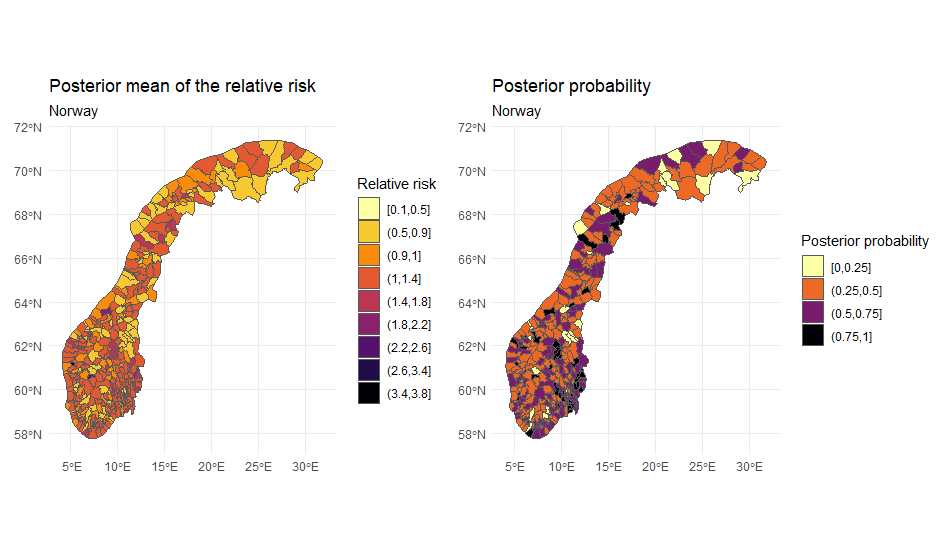
\includegraphics[width = \textwidth]{posterior_norway.png}
    \caption{Posterior mean of the area-specific risk and the posterior probability.}
    \label{posteriorNorway}
\end{figure}
% \begin{figure}[H]
%     \centering
%     \includesvg[width = textwidth]{posterior_norway.svg}
%     \caption{A negative binomial fit to the number of cases in Norwegian municipalities}
%     \label{nb_norge}
% \end{figure}
\clearpage
\section{Spatio-Temporal Models}
\subsection{Spatio-Temporal Models for Germany}
\subsection{Spatio-Temporal Models for Norway}
\section{Predictive Models}
\clearpage
\subsection{Predictive Models for Germany}
\subsection{Predictive Models for Norway}